\section{From calculus to efficient implementation}

It turns out that a variant of the $\mathsf{Linda}$ tuple space
\cite{DBLP:conf/parle/Gelernter89} where input is not blocking is the
critical innovation to an efficient implementation. Instead of
blocking we turn input from a key into the storage of a continuation
at the key. As the astute reader has already guessed, (the hashes of)
channels become keys.\\

%\begin{center}
\begin{figure}
  \centering
  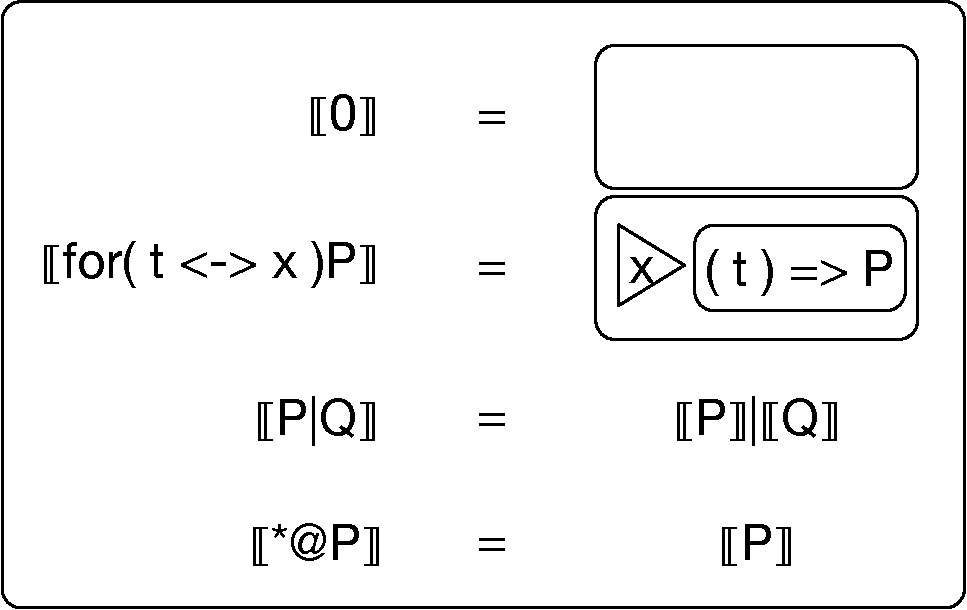
\includegraphics[scale=0.5]{MeTTaCalcImpl1.pdf} \\
  \caption{Compiler from $\mathsf{MeTTa}$-calculus to $\mathsf{RSpace}$}
\end{figure}
%\end{center}

Thus, the diagram above indicates how to turn a given process state
into an $\mathsf{RSpace}$ instance.

\begin{itemize}
  \item the first equation says that the $\pzero$ process corresponds
    to the empty $\mathsf{RSpace}$;
  \item the second says that a comprehension corresponds to an
    $\mathsf{RSpace}$ consisting of a single key-value pair; the key
    being the hash of the channel on which the comprehension is
    listening (the \emph{source} of the comprehension); and the value
    being the (multiset containing the single) continuation formed by
    created a pattern-matching style lambda from \emph{target} of the
    comprehension to its \emph{body}; \footnote{Sometimes we abuse the
      terminology and call the body the continuation.}
  \item the third equation translates the concurrent composition of
    two processes, say $P$ and $Q$, into the combination of their two
    $\mathsf{RSpace}$s using an operation $\mathsf{RSpace}$s on we
    define below.
\end{itemize}

\subsubsection{Parallel composition of $\mathsf{RSpace}$s}

If we are combining two $\mathsf{RSpaces}$ that only have a single
key-value pair, each; and the keys are not equal, then we simply
combing them into a single $\mathsf{RSpace}$ containing both key-value
pairs. More generally, when combining $\mathsf{RSpace}$s that have no overlap
in their key-sets, we simply return the $\mathsf{RSpace}$ whose
key-value pairs is the union of the key-value pairs of the
$\mathsf{RSpace}$s being combined.\\
 
\begin{figure}
  \centering
  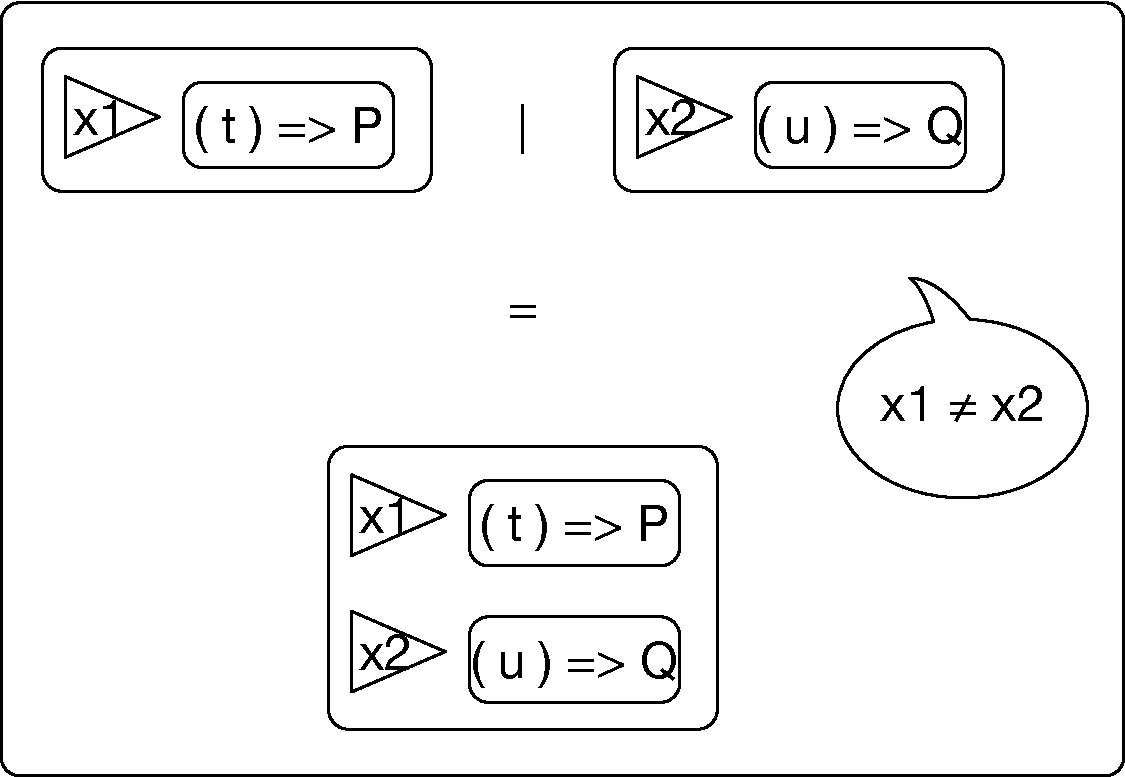
\includegraphics[scale=0.5]{MeTTaCalcImpl2.pdf}
  \caption{Compiler from $\mathsf{MeTTa}$-calculus to $\mathsf{RSpace}$ continued}
\end{figure}

When combining two $\mathsf{RSpaces}$ that only have a single
key-value pair, each, their keys are the same, but the patterns of
their continuations do not unify, then we simply combine them into a
single $\mathsf{RSpace}$ containing a single key-value pair, the key
of which is the key of each pair (remember, both pairs share a key)
and the value of which is the multiset containing the respective
values (continuations).

More generally, when combining $\mathsf{RSpace}$s that have overlap in
their key-sets, but the overlapping keys contain no continuations
whose patterns unify, we simply return the $\mathsf{RSpace}$ whose
key-value pairs is

\begin{itemize}
  \item the union of the key-value pairs of the $\mathsf{RSpace}$s
    being combined for the key-value pairs whose keys do not overlap;
  \item and constructs a new key-value pair for each pair in the
    overlap that shares a key, whose key is the key they share and
    whose value is the union of their respective multisets.
\end{itemize}

\begin{figure}
  \centering
  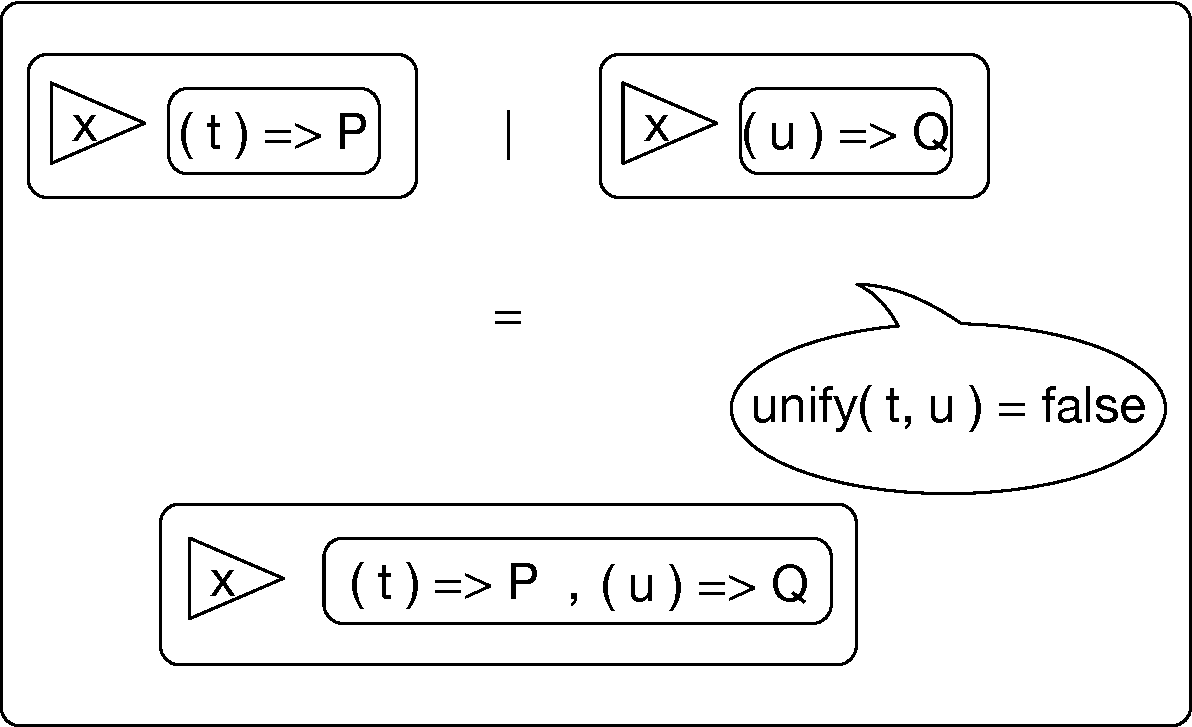
\includegraphics[scale=0.5]{MeTTaCalcImpl3.pdf}
  \caption{Compiler from $\mathsf{MeTTa}$-calculus to $\mathsf{RSpace}$ continued again}
\end{figure}

What remains is the case when combining two key-value pairs that have
unifying patterns in their multisets. The naive algorithm is quadratic
in the number of unification checks. However, $\mathsf{MORK}$ provides
a more efficient way to parallelize these checks.

[$\mathsf{MORK}$ algorithm description goes here.]
